\newpage
\section{Sheared Objects}

\subsection{ShearedCylinderHayterPenfold \cite{Hayter1984}}
\label{sect:ShearedCylinderHayterPenfold}
\hspace{1pt}\\

\begin{figure}[htb]
\begin{center}
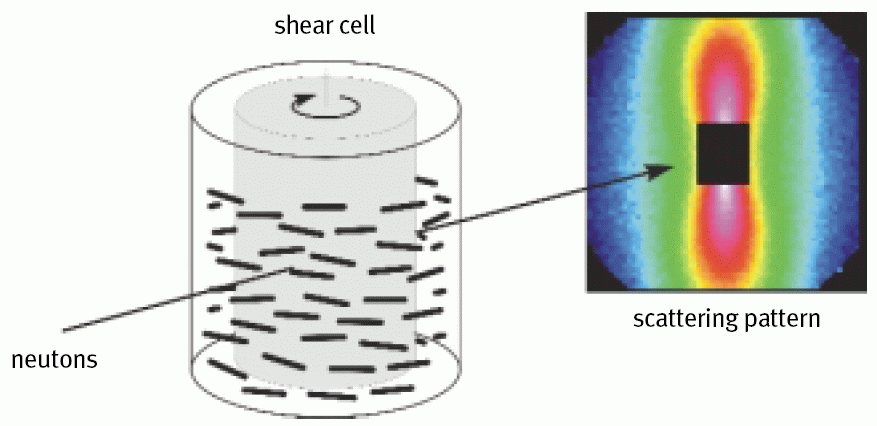
\includegraphics[width=0.7\textwidth,height=0.3\textwidth]{sheared_cylinders1.png}
\end{center}
\caption{Shear orientation of micelles in a shear cell with the
corresponding SANS-pattern.} \label{sheared_cylinders1}
\end{figure}

\begin{figure}[htb]
\begin{center}
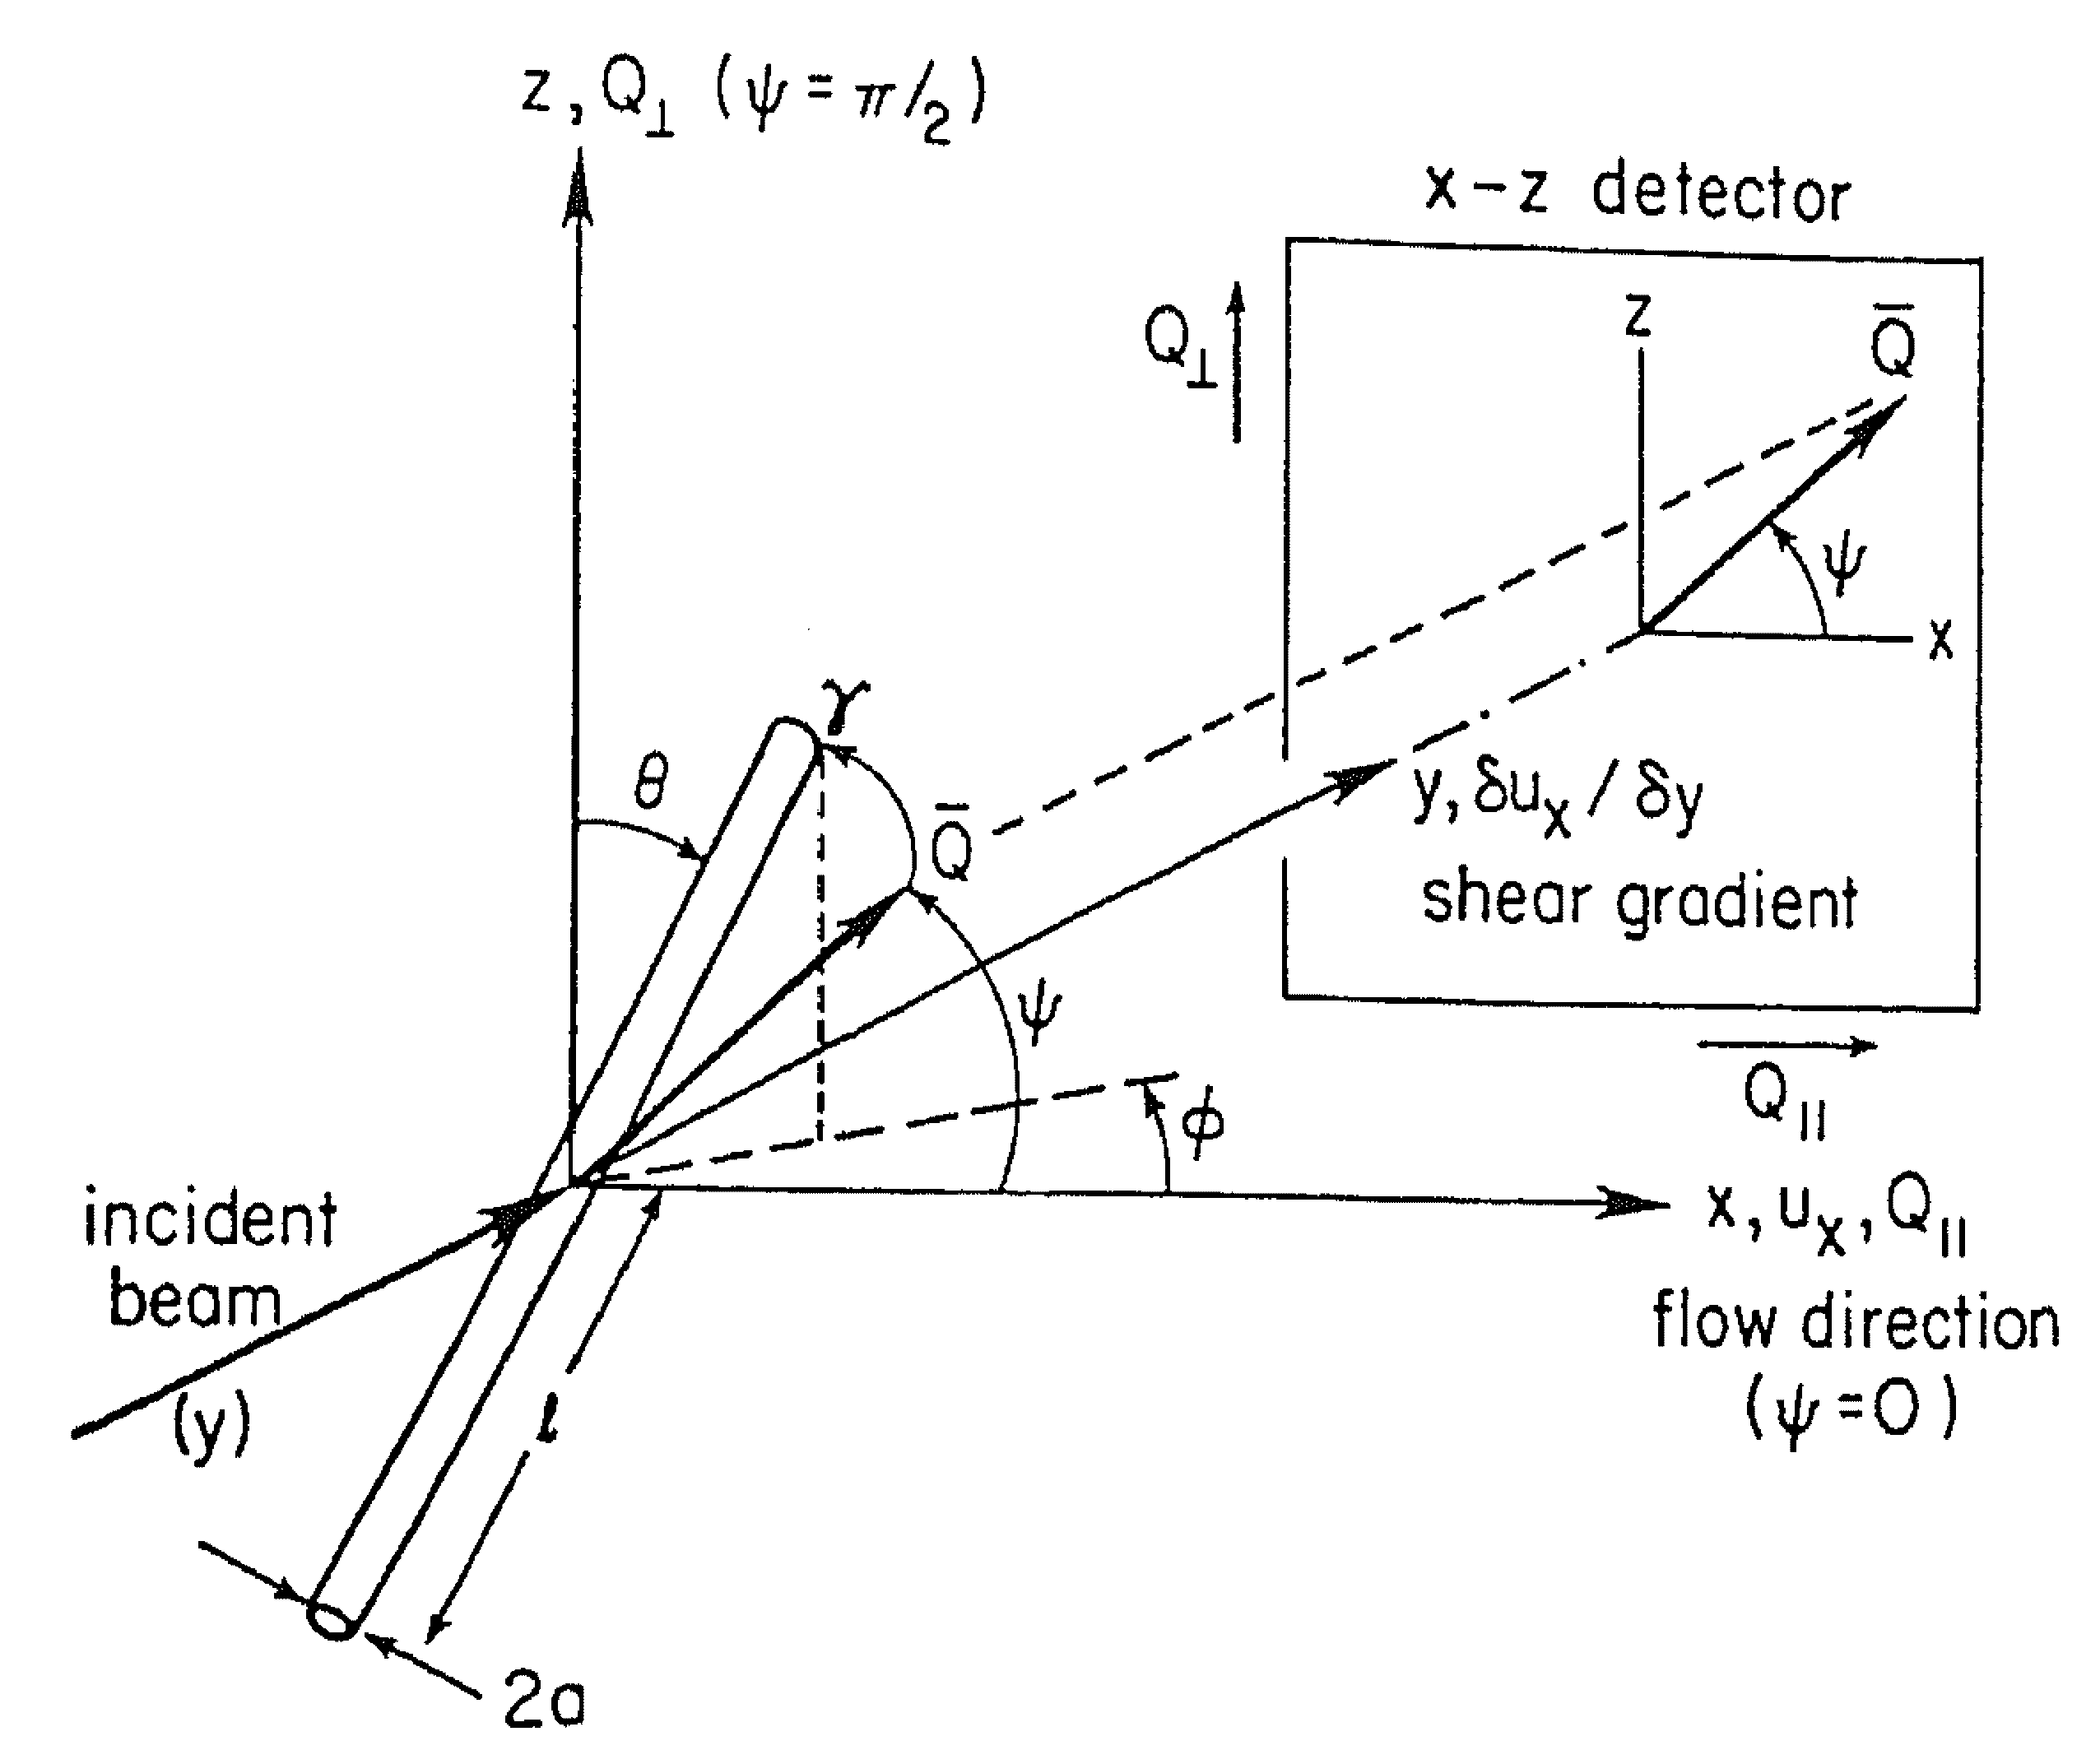
\includegraphics[width=0.7\textwidth,height=0.7\textwidth]{shear_cuette_SANS_geometry.png}
\end{center}
\caption{Cartesian and angular coordinates referred to the center
of a cylindrical micelle at origin. The relationship to the
spectrometer geometry is shown schematically. The momentum
transfer, $Q$, lies in the $z-x$ plane.}
\label{shear_cuette_SANS_geometry}
\end{figure}

The scattering from monodisperse dilute (non-interacting)
isotropic solution of anisotropic micelles is given by \BE I(Q) =
\left< \vert F(Q)\vert^2 \right>_Q \label{IQ_av} \EE where $F(Q)$
is the form factor for a micelle at a given orientation relative
to the momentum transfer $Q$ and $\left<\right>_Q$ denotes an
average over all such orientations.

For a uniform cylinder of length $L$ and diameter $2R$ the form
factor is given by:
\BE F(Q) = F(Q,\gamma) = 2\Delta\eta V
\frac{\sin\left(QL/2\cos\gamma\right)}{QL/2\cos\gamma}
\frac{J_1(QR\sin\gamma)}{QR\sin\gamma}
\EE
where $\gamma$ is the
angle between $Q$ and the cylinder axis, $V$ is the volume,
$\Delta\eta$ the scattering length density contrast relative to
the solvent, $J_1(x)$ is the first order Bessel function of the
first kind.

The scattering geometry for shear alignment is shown in Fig.
\ref{shear_cuette_SANS_geometry}. In general perfect alignment
will not be achieved, and an orientation distribution must be
employed such that the resultant scattering will be given by
\BE
I(Q,\psi) = \int_0^{2\pi}d\varPhi \int_0^\pi
p(\theta,\varPhi;\Gamma)\, \left(F^2(Q,\gamma^+)+F^2(Q,\gamma^-)
\right) \sin\theta d\theta
\EE
where
\begin{align}
\cos\gamma^\pm & = \sin\theta\cos\phi\cos\psi\pm\cos\theta\sin\psi \\[3mm]
p(\theta,\phi;\Gamma) & = \frac{(1-\cos
2\varPhi_0)(1+\sin^2\theta\cos 2\varPhi_0)^{3/2}}{4\pi\left[
1-\sin^2\theta\cos 2\varPhi_0\cos 2(\phi-\varPhi_0)\right]^2}
\end{align}
and
\BE
2\varPhi_0 = \arctan(8/\Gamma)
\EE
\begin{align}
\frac{\mathbf{Q}}{\abs{\mathbf{Q}}} &=
\begin{pmatrix}
\cos \psi \\
0  \\
\sin \psi
\end{pmatrix} \qquad
\frac{\mathbf{n}}{\abs{\mathbf{n}}} =
\begin{pmatrix}
\sin \theta \cos \phi \\
\sin \theta \sin \phi  \\
\cos \theta
\end{pmatrix} \\
\cos \angle(\mathbf{Q,n}) &= \cos \gamma = \frac{\mathbf{Q\cdot n}}{\abs{\mathbf{Q}}\abs{\mathbf{n}}} =  \cos\psi \sin\theta \cos\phi + \sin\psi \cos\theta
\end{align}

%[1] John B. Hayter and Jeff Penfold, Use of Viscous Shear Alignment
%To Study Anisotropic Micellar Structure by Small-Angle Neutron
%Scattering, J. Phys. Chem. 1984, 88, 4589-4593

%%%%%%%%%%%%%%%%%%%%%%%%%%%%%%%%%%%%%%%%%%%%%%%%%%%%%%%%%%%%%%%%%%%%%%%%%%%%%%%%%%

\newpage
\subsection{ShearedCylinderBoltzmann} ~\\

\begin{align}
p(\theta,\phi;\bar{\theta}) & = \exp(-\theta/\bar{\theta}) \\
\cos\gamma^\pm & = \sin\theta\cos\phi\cos\psi\pm\cos\theta\sin\psi
\end{align}

%%%%%%%%%%%%%%%%%%%%%%%%%%%%%%%%%%%%%%%%%%%%%%%%%%%%%%%%%%%%%%%%%%%%%%%%%%%%%%%%%%

\newpage
\subsection{ShearedCylinderGaussian}
\label{sect:ShearedCylinderGaussian}
~\\
\begin{align}
p(\theta,\phi;\bar{\theta}) & = \exp(-(\theta/\bar{\theta})^2) \\
\cos\gamma^\pm & = \sin\theta\cos\phi\cos\psi\pm\cos\theta\sin\psi
\end{align}

%%%%%%%%%%%%%%%%%%%%%%%%%%%%%%%%%%%%%%%%%%%%%%%%%%%%%%%%%%%%%%%%%%%%%%%%%%%%%%%%%%

\newpage
\subsection{ShearedCylinderHeaviside} ~\\

\begin{align}
p(\theta,\phi;\bar{\theta}) & = \Theta[\theta-\bar{\theta}] \\
\cos\gamma^\pm & = \sin\theta\cos\phi\cos\psi\pm\cos\theta\sin\psi
\end{align}

%\item[ShearedCylinderMaierSaupe] ~\\
%\begin{align}
%p(\theta,\phi;\bar{\theta}) & = \exp[\cos^2(\theta/\bar{\theta})]-1 \\
%\cos\gamma^\pm              & = \sin\theta \cos\phi \sin\psi \pm \cos\theta\cos\phi
%\end{align}
%
%\item[ShearedCylinderOnsager] ~\\
%\begin{align}
%p(\theta,\phi;\bar{\theta}) & = \exp[-\sin(\theta/\bar{\theta})] \\
%\cos\gamma^\pm              & = \sin\theta \cos\phi \sin\psi \pm \cos\theta\cos\phi
%\end{align}
